\section{Setup}
\begin{figure}[ht]
\centering
\import{qcm/figures/}{qcm_annotated_picture.pdf_tex}
\caption{Annotated picture of the prototype CF-QCM from above.  The
centrifuge is a standard swinging bucket type.}
\label{fig:cfqcmexpsetup}
\end{figure}

The CF-QCM experimental setup is shown in \Figure{fig:cfqcmexpsetup}.  It
consists of a \SI{25}{\milli\meter} diameter \SI{5}{\mega\hertz} gold
coated crystal in combination with an SRS QCM200 PLL based driver circuit
and an external rubidium frequency standard.  The driver circuit and
crystal are integrated into the arm of a commercial swinging bucket
centrifuge.  The QCM is then connected in proximity to a remote driver
which is tethered via a slip-ring connector to external data acquisition
electronics and a computer.  The crystal itself is mounted in a holder
such that the centrifugal force $F_\mathrm{c}$ is
always normal to the surface of the crystal.  On the sensing side of the
crystal is a $\SI{125}{\micro\liter}$ volume PDMS/glass cell containing the
sample.  The cell is made of a thin o-ring of PDMS (Sylgard 184, 10:1
ratio, cured \SI{20}{\minute} at \SI{120}{\celsius}),
outer diameter \SI{25}{\milli\meter}, inner diameter
\SI{15.5}{\milli\meter}, in
contact with the sensing side of the crystal and covered with
\SI{25}{\milli\meter} round N\raisebox{0.25em}{\relsize{-2}\b{o}}~1
coverglass of nominal thickness \SI{0.15}{\milli\meter}.  The non-sensing
side of the crystal remains in air and is isolated from the body of the
centrifuge.  

When in operation, the crystal and cell are mounted in either the
\textit{loading} configuration, where the centrifugal force is \textit{in
to} the sensing side or, by mounting it upside down, in the
\textit{unloading} configuration, where the force is \textit{away from} the
sensing side.

In addition to the standard QCM driver output, the computer simultaneously
records the angular velocity and internal temperature of the centrifuge
itself.  The angular velocity is obtained with an optical interrupter
switch placed over the spokes of an internal gear, acting as an ersatz
wheel encoder.  The temperature is obtained with a standard K-type
thermocouple.  The internal motor of the centrifuge was also interfaced to
an external DC power supply whose voltage was set by the same
computer, allowing the spin speed and acceleration of the centrifuge to be
controlled.
%We tried o-rings made of other stuff, but its just not as good as the PDMS.

\begin{figure}[ht]
\centering
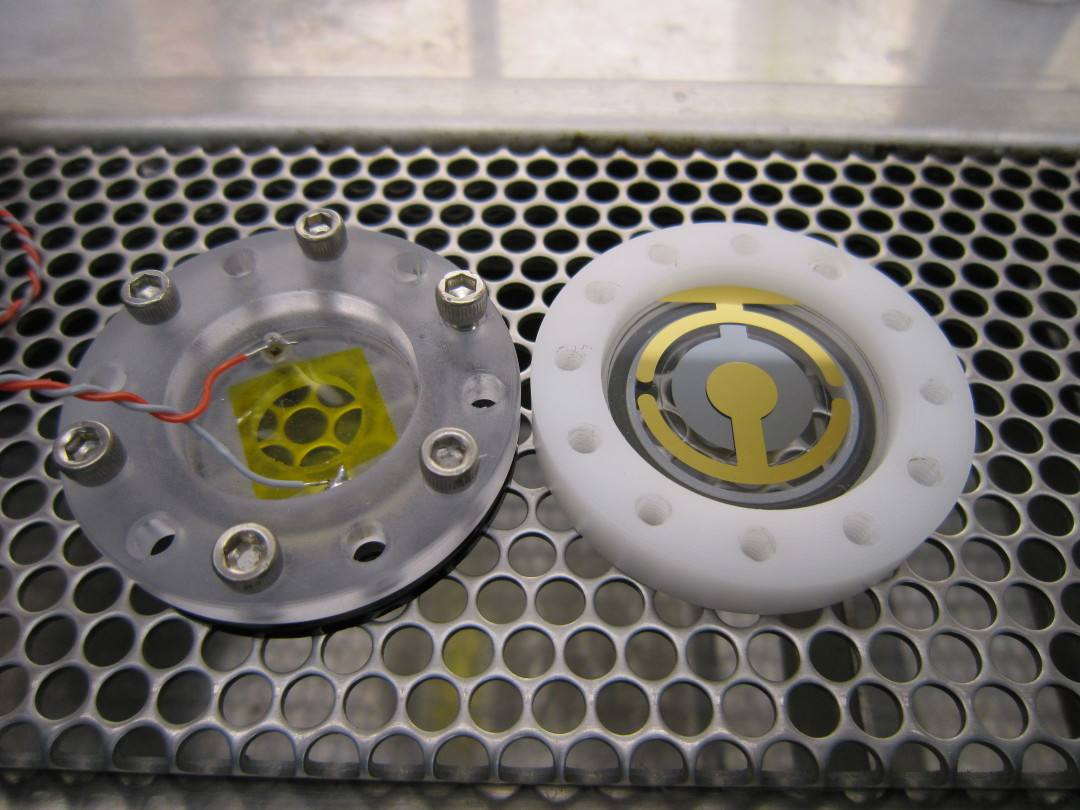
\includegraphics[width=10cm,keepaspectratio]{qcm/figures/qcm_holderdiss.jpg}
\caption{Holder for the crystal, shown split into its two halves.  The
crystal is inside the holder on the right.}
\label{fig:cfqcmexpsetup}
\end{figure}

\section{Noise and Comparison to QCM-D}\label{sec:suppqcmdcomp}
Typical of most QCM circuits, the QCM200 provides an output proportional to
$\df$, which is used directly in all discussions of $\df$.  However, unlike
a QCM-D device which gives a ``dissipation factor'', $D$, defined in
terms of the bandwidth $\dg$ as $D=2\dg/f_\mathrm{F}$, the QCM200
outputs the motional resistance $\Rm$ of the Butterworth van Dyke
equivalent circuit.  $\Rm$ is, related to
the bandwidth $\Gamma$ and the QCM-D dissipation $D$ by 
\begin{align}
 \Rm&=\left(4 \pi \Lm\right) \Gamma\\
 &=\left(2 \pi \Lm f_\mathrm{F}\right) D,
\end{align}
where $\Lm$ is the Butterworth van Dyke equivalent motional inductance.
Because of the small load approximation, $\df/f_\mathrm{F} \ll 1$ and
likewise $\Delta L/\Lm \ll 1$, $\Lm$ can effectively be treated as a
constant~\cite{geelhood2002transient}.  The motional inductance $\Lm$ is
typically in the range of
\SI{30}{\milli\henry}~\cite{srsqcm200manual}~\cite{hussain2005ots} to
\SI{40}{\milli\henry}~\cite{gottschling2000detection}~\cite{arnau2002circuit}~\cite{snellings2001response},
with \SI{40}{\milli\henry} being more common and the value used in the
present analysis.  At $\Lm=\SI{40}{\milli\henry}$, the instrument recorded
$\Rm=\SI{359}{\ohm}$ in water, which is within \SI{1}{\percent} of the
predicted value~\cite{kanazawa1985frequency} of \SI{357}{\ohm}.  In this
sense, dissipation $D$ and motional resistance $\Rm$ are independent but
equivalent measures of the QCM bandwidth.

The noise was calculated in $\df$ and $\Rm$ by obtaining the standard
deviation of the output signal at constant acceleration.  For the SRS
QCM200 employed in the experiment the noise was measured at
\SI{0.4}{\hertz} (\SI{0.008}{ppm}) for $\df$ and \SI{0.006}{\ohm}
(\SI{13}{ppm}) for $\Rm$, corresponding to a signal to noise ratio of
\SI{110}{\decibel}.  The measured noise is close to the manufacturer's
specification~\cite{srsqcm200manual} of \SI{0.1}{\hertz} for $\df$ and
$\pm\SI{28}{ppm}$ for $\Rm$.  The noise was further analyzed for both the
loading and unloading orientations of the crystal, as well as for different
centrifuge spin speeds.  In either case, no discernible difference in the
noise was observed.  At no point was the centrifuge or bucket assembly
modified in an attempt to try and reduce system noise.

In comparison, a typical QCM-D such as those sold by
Q-Sense\footnote{BiolinScientific / Q-Sense, Hängpilsgatan 7, SE-426 77
Västra Frölunda, Sweden,  \url{http://www.q-sense.com/}} will have noise of
about \SI{0.3}{\hertz} in $\df$ and \num{0.2e-6} in $D$ at
\SI{5}{\mega\hertz}~\cite{su2005comparison}~\cite{peh2007understanding}.
Converting from $\Rm$ to $D$ and vice-versa, the SRS QCM200 has an
equivalent noise in $D$ of \num{0.005e-6} and the Q-Sense QCM-D an
equivalent noise in motional resistance of \SI{0.25}{\ohm}.  In terms of
$\dg$, the Q-Sense QCM-D has a noise of \SI{0.5}{\hertz} and the SRS QCM200
\SI{0.01}{\hertz}.  Even though the chosen value for $\Lm$ gives $\Rm$
within \SI{1}{\percent} of the predicted value for water, uncertainties in
the value of $\Lm$ used for the $\Rm$-$\dg$ conversion do not significantly
affect the analysis for the range of $\Lm$ values quoted in the literature.

It is clear that the SRS QCM200 PLL based driver and a QCM-D device are
both measures of the same underlying physical phenomena taking place in a
resonating quartz crystal~\cite{geelhood2002transient}.  It is important to
note that the important aspect of the CF-QCM, the centrifugal force, is
independent of the type of technique used to drive and monitor the quartz
crystal.  There is no reason why the CF-QCM technique would not apply to
all QCM based measurement techniques.  

\section{Environmental Effects and Noise}
In the next chapter is presented the response of the CF-QCM under different
load situations.  Before doing so, it is prudent that all non-sample
phenomena which could influence the sensorgram are taken into account.  Such
phenomena have been tabulated in \Table{tbl:environmentaleffects}.
\begin{table}[ht]
\centering
\begin{tabular}{l>{\raggedright}p{10cm}l}
\toprule
\textbf{phenomena} & \textbf{response} & \textbf{refs}\tabularnewline%
\midrule
temperature & \SI{8}{\hertz\per\celsius} and \SI{4}{\ohm\per\celsius} in water
&\cite{srsqcm200manual}\tabularnewline%
 & Third order polynomial with maximum around \SI{24}{\celsius} with
$a_1=\num{2.3888}$, $a_2=\num{-1.8719e+02}$, $a_3=\num{4.8587e+03}$,
$a_4=\num{-4.1814e+04}$. &\cite{reipa2006long}\tabularnewline%
electric field & negligible  &\cite{walls1995fundamental}\tabularnewline%
magnetic field & \SI{10}{\per\tesla} for fields smaller than \SI{10}{\tesla} &\cite{walls1995fundamental}\tabularnewline%
pressure & \SI{-2970}{\hertz\centi\meter\squared\per\kilo\gram} for changes to \SI{+2.1}{\kilo\gram\per\centi\meter\squared} &\cite{reipa2006long}\tabularnewline%
 & \SI{-1458}{\hertz\centi\meter\squared\per\kilo\gram} (\SI{10}{\mega\hertz} crystal) &\cite{heusler1988measurement}\tabularnewline%
mechanical stress & $\Delta f = 1.62 g_f^{1.72}$ for two point symmetrical mounting in air &\cite{fletcher1979comparison}\tabularnewline%
sedimentation potential &  & \tabularnewline%
parasitic capacitance & \SI{2}{\hertz\per\pico\farad} &\cite{srsqcm200manual}\tabularnewline%
& \SI{0.825}{\hertz\per\pico\farad} (BvD analysis) & [~] \tabularnewline%
acceleration & \SI{9e-11}{\per g}, depending on orientation &\cite{norton1993tactical}\tabularnewline%
 & \SI{0.0218813}{\hertz\per g} in air &\cite{1536938}\tabularnewline%
\bottomrule
\end{tabular}
\caption{Environmental effects on the QCM resonance frequency.}
\label{tbl:environmentaleffects}
\end{table}

From \Table{tbl:environmentaleffects} it is apparent that the dominant
source of signal \textit{drift} will be due to the inherent temperature
dependent viscosity of water.  This is a good thing, because temperature
drift can be a rather slow process compared with other types of signals.
To evidence this, a parametric plot of g-force verses temperature
for a typical run, total time \SI{200}{\second}, is shown in
\Figure{fig:qcmairtime} for both air and water.  In both cases 
the temperature increases as the centrifuge spins.  However,
the temperature drifts are extremely small during the course of a run, less
than \SI{0.1}{\celsius}.
\begin{figure}[ht]
 \centering
 \import{includes/}{setpgfinc}
 \import{qcm/figures/}{showtempairwater}
 \caption{Parametric plot showing temperature drift during an experimental
	run from 0 to \SI{90}{g} and back, taking \SI{200}{\second}.}
\label{fig:qcmairtime}
\end{figure}
